\chapter{Discussão e Atividades}

\section{Emulador RST}

O primeiro passo para começarmos a desenvolver o projeto era criar uma representação do sinal trifásico, para que este sirva de referência para os testes futuros.

A principio, sabemos que os sinais trifásicos possuem defasagem de 120º entre cada onda e oscilam a 60Hz, sendo assim, é necessário criar uma máquina sequencial que seja capaz de gerar tal sinal.

\begin{figure}[!htp]
	\centering
	\caption{Sinais RST}
	\fbox{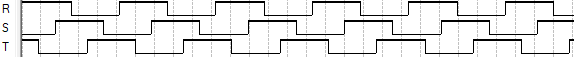
\includegraphics[width=16cm]{images/sinalRST}}
	\label{fig:sinais-rst}
\end{figure}Discu\303\247\303\2

O primeiro passo foi elaborar um diagrama de sequência que satisfaça as condições para a geração dos sinais.

\begin{figure}[!htp]
	\centering
	\caption{Diagrama de Estado Emulador RST}
	\fbox{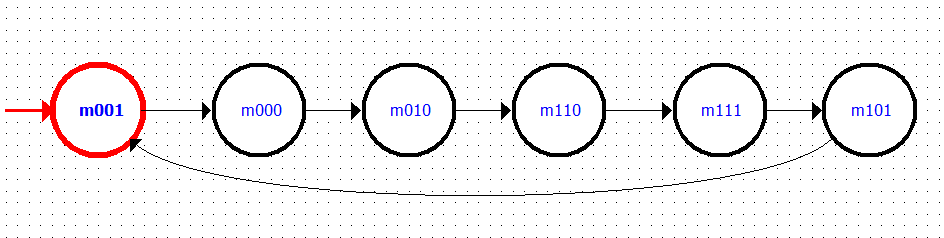
\includegraphics[width=16cm]{images/disgrama-de-estado-EmuladorRST}}
	\label{fig:disgrama-de-estado-EmuladorRST}
\end{figure}

Para a construção deste diagrama foi utilizado três bits para referenciar os estados, note que de um estado para outro apenas um bit é alterado, foi feita esta escolha pelo fato de que com isso a implementação do circuito iria ser simplificada. Montando a tabela de próximos estados e de excitação dos flip-flops.

\begin{figure}[!htp]
	\centering
	\caption{Tabela de estados e excitação dos Flip-flops Emulador RST}
	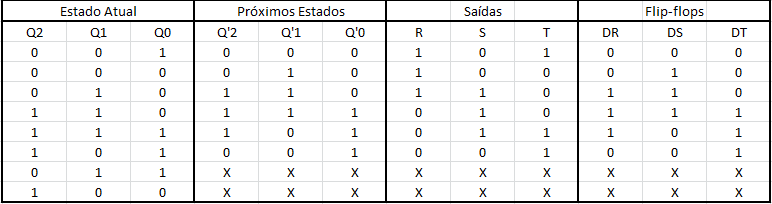
\includegraphics[width=16cm]{images/tabela-RST}
	\label{fig:tabela-RST}
\end{figure}

Utilizando Karnaugh para fazer a simplificações e encontrar as expressões de cada saída do circuito, encontramos que:

$$DR = Q1$$
$$DS = \overline{Q0}$$
$$DT = Q2$$

As saídas serão:

$$R = \overline{Q2}$$
$$S = Q1$$
$$T = Q0$$

A partir disto podemos construir o circuito do emulador RST, representado pela Figura \ref{fig:circuito-RST}.

\begin{figure}[!htp]
	\centering
	\caption{Circuito do Emulador RST}
	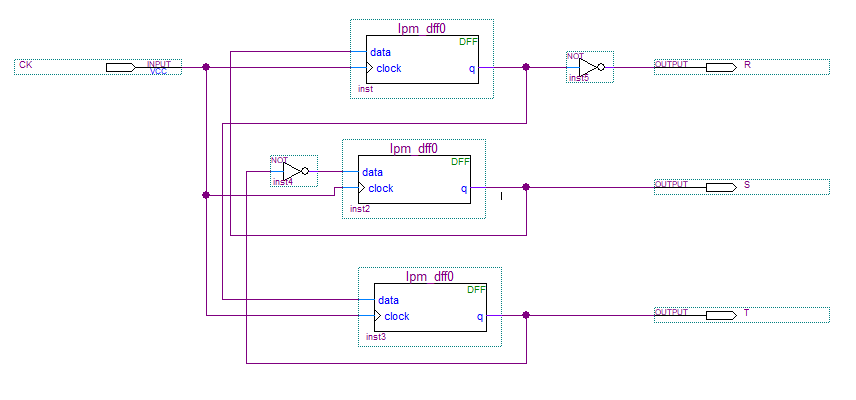
\includegraphics[width=16cm]{images/circuito-RST}
	\label{fig:circuito-RST}
\end{figure}

Tal circuito está gerando sinais periódicos defasados em 120º, porém apenas com isto não é possível que elas oscilem a 60Hz, pois a placa em que foram feito os teste possuí clock de 25.175MHz, portanto, é necessário reduzir o clock de entrada de tal circuito. 

Para fazer tal redução foi utilizado a saída Carry-out de um contador de módulo 34965 como o clock do nosso circuito RST, com isso o clock será dividido pelo módulo do contador. Mas isso ainda não é suficiente para alcançar os 60Hz, para atingir o valor correto foi inserido um flip-flop do tipo T para dividir o clock por dois, fazendo com que entre no circuito um sinal de 360Hz que será dividido por seis ao passar pelo emulador RST, devido ao fato desta ter 6 estados. Assim teremos os sinais RST a 60Hz.

A Figura \ref{fig:circuito-RST-complete} representa o circuito que gerará os sinais corretamente.

\begin{figure}[!htp]
	\centering
	\caption{Circuito do Emulador RST com saídas a 60Hz}
	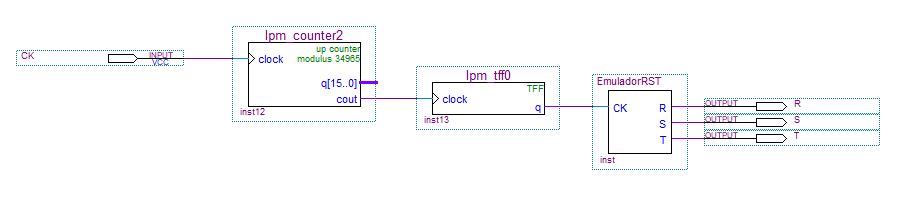
\includegraphics[width=16cm]{images/circuito-RST-complete}
	\label{fig:circuito-RST-complete}
\end{figure}

\section{Medidor de Período}

Primeiramente precisamos ser capazes de receber um sinal de entrada e interpreta-lo para que seja possível dizer qual das três fases foi inserida, então é necessário criar um circuito capaz de identificar qual é o período da fase inserida, representado pela Figura \ref{fig:diagrama-medidor-de-frequencia}.

\begin{figure}[!htp]
	\centering
	\caption{Diagrama esquemático do medidor de período da fase de referência}
	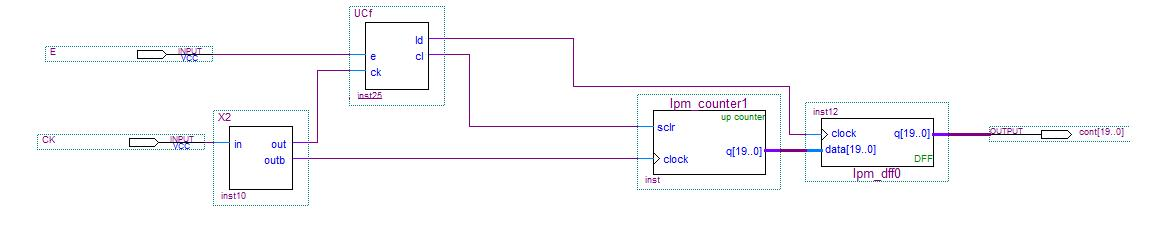
\includegraphics[width=16cm]{images/diagrama-medidor-de-frequencia}
	\label{fig:diagrama-medidor-de-frequencia}
\end{figure}

Sabendo que o período é toda a extensão desde sua primeira
borda de subida até a sua próxima borda de subida, então, para conseguir identifica-lo, foi utilizado um contador que irá contar o número de clocks dentro de um período e então armazena-lo em um registrador.

Ao inicio de cada período o contador é zerado através do sinal Cl da unidade de controle UCf, tal circuito será explicada mais a frente. no mesmo clock, através do sinal Ld o ultimo valor contado é transferido para o registrador, para que ambos comandos sejam executados em ordem correta foi criado a unidade X2.

\begin{figure}[!htp]
	\centering
	\caption{Unidade X2}
	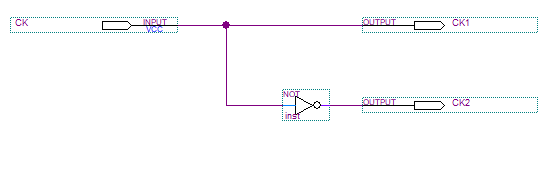
\includegraphics[width=16cm]{images/unidade-x2}
	\label{fig:unidade-x2}
\end{figure}

A única função da unidade da Figura \ref{fig:unidade-x2} é, a partir de uma entrada, no caso o clock, gerar duas saídas, uma idêntica ao sinal de entrada e a outra com o sinal negado.

Note que, o clock do contador provem do sinal CK2 de X2, ou seja, tal contador trabalha na borda de descida do clock original, devido a isto os comandos Cl e Ld podem ser feitos no mesmo clock, uma vez que, assim que forem gerados sinais altos de Cl e Ld, na borda de subida do clock, o valor contado pelo contador é salvo no registrador e no borda de descida deste mesmo clock, é feito o clear do contador.

\section{Correção de Erro aleatório}

Utilizando a unidade X2 para sincronizar os comandos faz com que exista a geração de um erro aleatório, possuindo dois casos extremos.

\begin{itemize}	
	\item Exite o caso em que o sinal de entrada é inserido exatamente antes da borda de subida do clock, então a zeragem do contador possuirá um atraso de 0,5 clock, ou seja, um erro de -0,5 clock, porém note que no valor registrado é desconsiderado 0,5 clock, com isto é gerado mais um erro de -0,5 clock, mostrado na Figura \ref{fig:erro-leitura1};
\end{itemize}

\begin{figure}[!htp]
	\centering
	\caption{Entrada exatamente antes da borda de subida}
	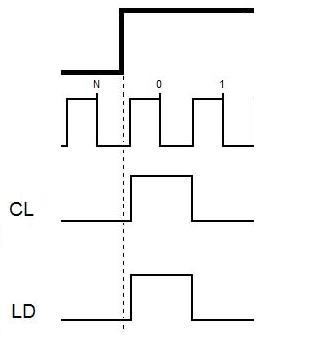
\includegraphics[width=7cm,height=7cm]{images/erro-leitura1}
	\label{fig:erro-leitura1}
\end{figure}

\clearpage

\begin{itemize}	
	\item No caso em que o sinal de entrada é inserido exatamente depois da borda de subida do clock, o contador será zerado com um atraso de 1,5 clocks, ou seja, com um erro de -1,5 clocks. Além disto o valor é registrado com 1 clock a mais, gerando um erro de +0,5 clock na leitura, representado pela Figura \ref{fig:erro-leitura2}.
\end{itemize}

\begin{figure}[!htp]
	\centering
	\caption{Entrada exatamente depois da borda de subida}
	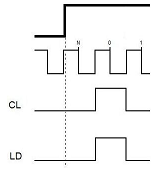
\includegraphics[width=7cm,height=7cm]{images/erro-leitura2}
	\label{fig:erro-leitura2}
\end{figure}

Analisando todas as combinações de erros possíveis nos dois casos extremos e utilizando a operação de convolução para estimar a probabilidade conjunta do dois eventos (carga e zeragem), entao, pode-se concluir que há a geração de um erro aleatório do qual varia de acordo com uma distribuição de probabilidade contínua com centro em -1 e bordas em -2 e 0. A Figura \ref{fig:distribuicao-de-probabilidade-do-erro} representa tal distribuição.

\begin{figure}[!htp]
	\centering
	\caption{Distribuição de probabilidade do erro}
	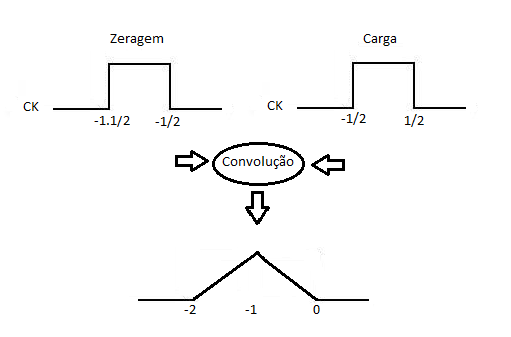
\includegraphics[width=14cm,height=10cm]{images/distribuicao-de-probabilidade-do-erro}
	\label{fig:distribuicao-de-probabilidade-do-erro}
\end{figure}

Note que, pelo fato da distribuição ter centro em -1, então o erro mais provável é o de -1 clock, ou seja, a cada leitura será perdido um clock da fase de entrada, fazendo com que as medições utilizem dados incorretos. O ideal nesta situação é que o centro da curva de distribuição de probabilidade seja exatamente em 0, assim o erro mais provável será de 0 clocks, tendo assim uma leitura mais correta da fase de entrada.

No primeiro circuito, o contador possuía uma entrada sclr (Synchronous Clear), este comando permitia zerar todos os bits do contador, porém, para corrigir tal problema alterou-se esta entrada para um sset (Synchronous set), este comando irá inserir um valor preestabelecido, no caso, será inserido o valor 1.

Desta forma iremos inserir um erro de +1 clock na leitura, uma vez que o primeiro clock não será contado, e sim inserido, porém, isso faz com que a distribuição de probabilidade atinja o comportamento ideal, ou seja, somando 1 ao erro aleatório o centro da curva ficará em 0, representado pela Figura \ref{fig:distribuicao-de-probabilidade-do-erro1}.

\begin{figure}[!htp]
	\centering
	\caption{Distribuição de probabilidade do erro com centro em 0}
	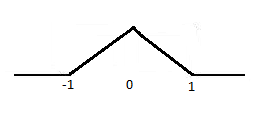
\includegraphics[width=8cm,height=5cm]{images/distribuicao-de-probabilidade-do-erro1}
	\label{fig:distribuicao-de-probabilidade-do-erro1}
\end{figure}

Note que esta solução não corrige todo o problema apenas diminui a probabilidade de erros, o ideal seria que não houvessem erros na leitura. Para que seja possível garantir que o sinal lido é confiável foi criado um outro circuito que visa promover isto, tal circuito será apresentado mas a frente.

\section{Gerador}

O circuito atual é capaz de medir o período de um sinal de entrada, porém, tudo será perdido se o sinal for retirado, o próximo passo então é criar um circuito capaz de gerar um sinal em sincronismo com o sinal de referência recebido. 

Primeiramente foi construído um diagrama de estado para uma UC (Unidade de Controle) capaz de gerenciar os componentes do circuito com o objetivo de fazer a cópia do sinal recebido, representada pela Figura \ref{fig:diagrama-de-estado1}.

\begin{figure}[!htp]
	\centering
	\caption{Diagrama de estados da nova UC}
	\fbox{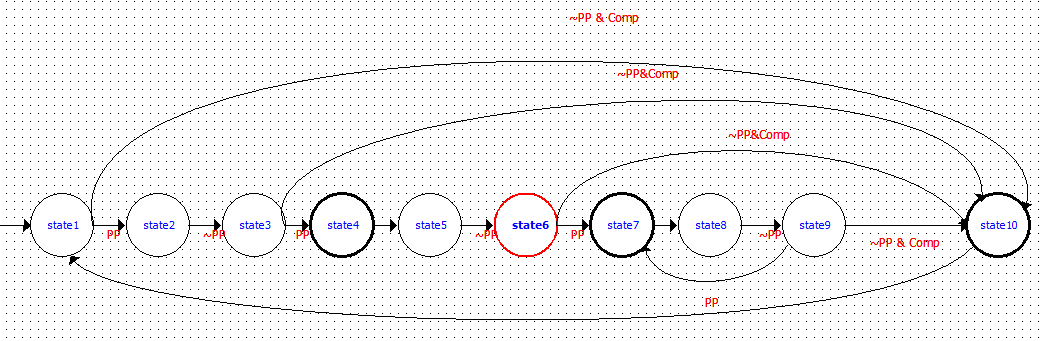
\includegraphics[width=16cm]{images/diagrama-de-estado1}}
	\label{fig:diagrama-de-estado1}
\end{figure}

Ao conectar um sinal de entrada ao circuito, este começará no estado 1 e então irá para o estado 2 quando PP (sinal de entrada) estiver em 1. Para passar para o estado 3 é necessário que PP esteja em 0. Note que este processo é feito para ignorar o primeiro período já que ele pode não ser um sinal muito confiável, devido ao fato de não sabermos se o sinal lido inicialmente está exatamente no inicio de um período da fase.

Chegando ao estado 4, o sinal Cl ficará em nível alto, limpado assim o contador, em seguida passa-se para o estado 5, em que, junto com o estado 6 irão esperar passar outro período, chegando finalmente no estado 7, em que são gerados sinais Cl e Ld. Garantida esta primeira medição correta do período, a máquina evolui sucessiva e repetidamente pelos estados 8, 9 e de volta para o 7, onde são providos os sinais Cl e Ld, permitindo a realização de novas e corretas medições, até que o sinal de entrada for retirado e o sinal Comp esteja em 1.

O sinal Comp irá ficar em 1 sempre que o contador atingir o valor lido nos estado 4, 5 e 6, ou seja, quando completar um período da fase de entrada.

Indo para o estado 10, onde é gerado um sinal Cl para manter o sincronismo com a fase lida e então passa para o estado 1. A partir deste ponto o a maquina fica repetidamente indo do estado 1 para o 10, esta transição irá ocorrer sempre que o sinal de entrada estiver em 0 e o Comp estiver em alto, ou seja, sempre ao fim de um período.

A partir deste diagrama de estado podemos construir o circuito da Figura \ref{fig:gerador}. Note que parte do circuito foi reaproveitado, o contador e o registrador. O comparador abaixo (inst 11) faz a comparação entre o sinal corrente e o valor de frequência armazenado, gerando assim o sinal Comp que é utilizado pela UC. Tal sinal, possui um ciclo ativo muito pequeno, que impede a visualização deste em um osciloscópio, a fim de gerar um sinal capaz de ser visualizado foi inserido o comparador na parte superior (inst 10), que irá comparar a contagem em curso com a metade da contagem registrada que será obtido do registrador de deslocamento ao lado (inst 5), fazendo com que o sinal "copia" de saída possua ciclo ativo de 50\% síncrono com o sinal de entrada.

\begin{figure}[!htp]
	\centering
	\caption{Diagrama de estados da nova UC}
	\fbox{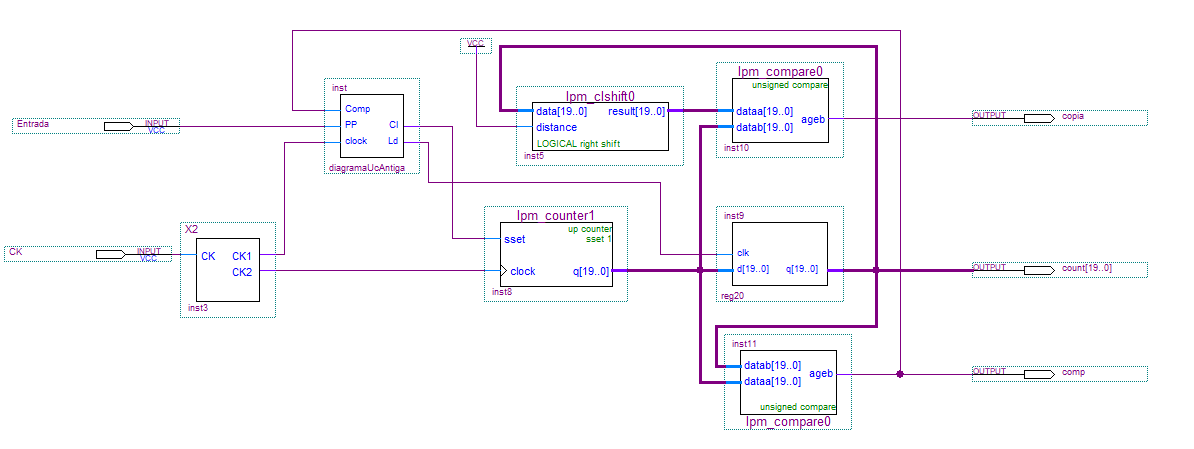
\includegraphics[width=16cm,height=7cm]{images/gerador}}
	\label{fig:gerador}
\end{figure}

\section{Comparador de Fase}



Para utilizar o método de comparação de fases requer uma frequência de seis vezes a frequência da fase de referência. Assim, o contador Ipm\_counter3 (inst) gera esta frequência dividindo o clock por seis, sendo então utilizado para realizar uma contagem entre as bordas de subida da fase de referência pelo contador Ipm\_counter5 (inst2), resultando em uma contagem truncada em $\frac{1}{6}$ do período da fase de referência, sendo armazenada em um registrador Ipm\_dff1 (inst3) pelo pulso Ld.

Como o contador Ipm\_counter5 (inst2) recebe um clock com $\frac{1}{6}$ da
frequência original do circuito, é utilizado um Clear assíncrono que ocorre na borda de descida anterior ao pulso Cl, com metade de sua duração, proveniente da porta "E" AND2 (inst10) entre o pulso Cl e o flip-flop tipo D DFF (inst9), que também realiza o Clear na máquina comparadora de fases.

O comparador Ipm\_compare (inst4) provém então o clock necessário para a
máquina comparadora de fases, e realiza também o Clear do contador Ipm\_counter4 (inst1), através da comparação entre a contagem truncada em $\frac{1}{6}$ do período da fase de referência e a do próprio contador, após o atraso de meio período de clock, obtido com o flip-flop tipo D DFF (inst9), pois sua saída também ocorre em uma borda de descida. Como uma divisão por seis pode envolver resto, o contador Ipm\_counter4 (inst1) também recebe outro sinal de Clear através da porta "OU" OR2 (inst5) produzido a cada período da fase de referência, evitando-se o acúmulo de erros.
